\chapter{Cenni sulla sintesi dei filtri analogici e filtri numerici}

\begin{figure}[h]
    \centering
    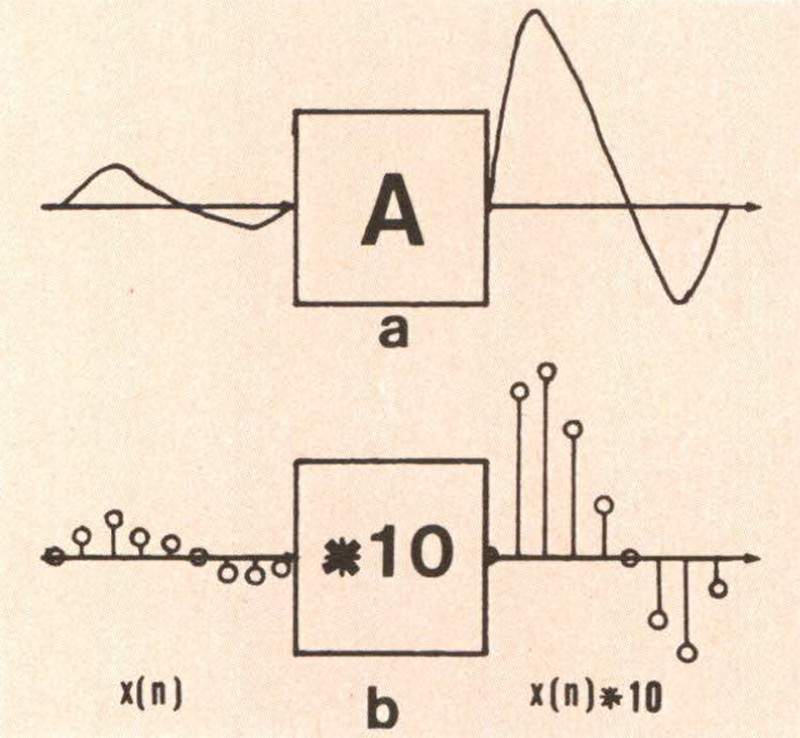
\includegraphics[scale = 0.5]{Filtro analogico e filtro numerico esempio.jpg}
\end{figure}  

\newpage 

\section{Sintesi di un filtro}

Idelmente, si progetta un filtro per eliminare parte del contenuto armonico di un segnale, 
lasciandone inalterata la porzione restante. \newline 

L'intervallo di frequenze del segnale in cui il filtro nominalmente non apporta delle modifiche  
prende il nome di banda passante del filtro. \newline 

Un filtro, in base al suo scopo, viene definito come: 

\begin{itemize}
    \item filtro passa-basso 
    \item filtro passa-alto 
    \item filtro passa-banda 
\end{itemize} 

Un filtro ideale dovrebbe essere caratterizzato da una funzione di trasferimento unitaria all'interno della banda passante, 
mentre la funzione di trasferimento dovrebbe essere identicamente nulla all'esterno della banda passante. \newline 

In altri termini, il filtro non dovrebbe attenuare le frequenze desiderate, 
mentre l'attenuazione dovrebbe essere infinita per quelle indesiderate. \newline 

Grazie alla definizione e spiegazione di cosa è un filtro, 
possiamo scrivere che è importante sia lo spettro di ampiezza della funzione di trasferimento 
che lo spettro di fase. \newline 

Idealmente, un filtro dovrebbe introdurre un ritardo costante su tutte le componenti armoniche entro la banda passante, 
e questo si traduce, notorialmente, in un andamento lineare della sua caratteristica di fase nello stesso intervallo 
di frequenze. \newline 

Il comportamento ideale, riguarda la transizione brusca da banda passante (in inglese pass band) 
a banda eliminata (stop band) può essere approssimato da un filtro reale. \newline 

La sintesi di un filtro comincia con l'assegnazione della cosiddetta "maschera" (mask) del suo spettro di ampiezza. \newline 

La maschera contiene le informazioni sul comportamento del filtro (quindi se è un filtro passa-alto, passa-basso, passa-banda) 
e le tolleranze ammissibili. \newline 

Siccome il comportamento ideale non portrà mai essere conseguito, si accettano i seguenti criteri: 

\begin{itemize}
    \item lo spettro di ampiezza (cioè il modulo della funzione di trasferimento) del filtro presenti una oscillazione (ripple) residua all'interno della banda passante 
    \item la regione di transizione da banda passante a banda eliminata abbia estensione non nulla 
    \item il comportamento in banda eliminata possa essere non ideale, con una oscillazione intorno allo zero, ovvero con una tendenza asintotica a zero 
\end{itemize}

La maschera del filtro, impostata in fase di progetto, specifica i margini di accettibilità delle non idealità elencate. \newline 

\newpage 

\subsection{Esempi di filtri passa-basso} 

\begin{figure}[h]
    \centering
    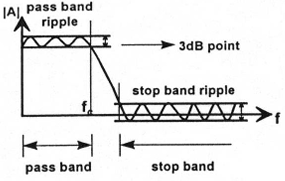
\includegraphics[scale = 1]{Sintesi di un filtro passa-basso.PNG}
\end{figure}  

Questo è un esempio di una maschera di un filtro passa-basso. \newline 

Possiamo notare che: 

\begin{itemize}
    \item il valore del guadagno in banda passante, idealmente dovrebbe essere uguale a uno, ma nella realtà può essere maggiore di 1 se il filtro amplifica o minore di 1 se il filtro attenua 
    \item la frequenza di taglio $f_c$ del filtro, definita come il valore di frequenza per cui il guadagno è sceso di $\frac{1}{\sqrt{2}} = 0.707$ volte il valore nominale all'interno della banda passante. \\ 
    In altri termini, considerando il guadagno del filtro $\abs{A_0}$ si ha dunque $\abs{H(f_c)} = \frac{A_0}{\sqrt{2}}$ o, usando i db, $\abs{H(f_c)}_{db} = \abs{A_0}_{db} - 3_{db}$ 
\end{itemize}

Un filtro passa-basso di questo tipo può essere sintetizzato, quindi progettato e fisicamente realizzato, assemblando insieme componenti resistivi, capacitivi e induttivi, 
scegliendo a priori la frequenza di taglio desiderata. \newline 

Ci sono diverse famiglie di filtri. \newline 

Un esempio di famiglia di filtri passa-basso sono i filtri di Butterworth. \newline 

L'andamento del modulo, per questa famiglia di filtri, è del tipo: 

{
    \Large 
    \begin{equation}
        \abs{H_n (f)} = \abs{A} = \frac{1}{\sqrt{1+(\frac{f}{f_c})^{2n}}}
    \end{equation}
}

dove n è un numero intero e indica l'ordine del filtro: il suo valore determina l'estensione della regione di transizione da banda passante a banda eliminata. \newline 

Di seguito, il modulo, la fase e la realizzazione di un filtro di Butterworth: 

\begin{figure}[h]
    \centering
    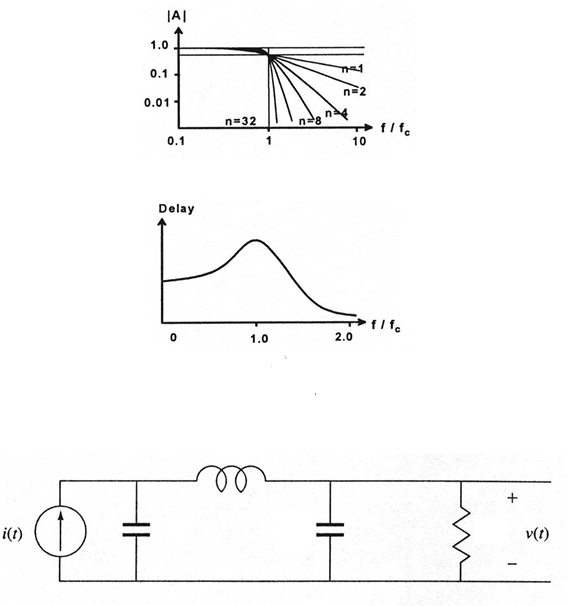
\includegraphics[scale = 1]{Realizzazione e progettazione di un filtro di Butterworth.PNG}
\end{figure}  

Un'altra famiglia di filtri passa-basso sono i filtri di Chebyshev. \newline 

Un filtro di Chebyshev è caratterizato da un andamento dello spettro di ampiezza esprimbile come : 

{
    \Large 
    \begin{equation}
        \abs{H_n (f)} = \frac{1}{\sqrt{1 + \varepsilon_p C_n ^{2} (\frac{f}{f_s})}}
    \end{equation}
} 

\newpage 

Di seguito, lo spettro delle ampiezze di due filtri Chebyshev: 

\begin{figure}[h]
    \centering
    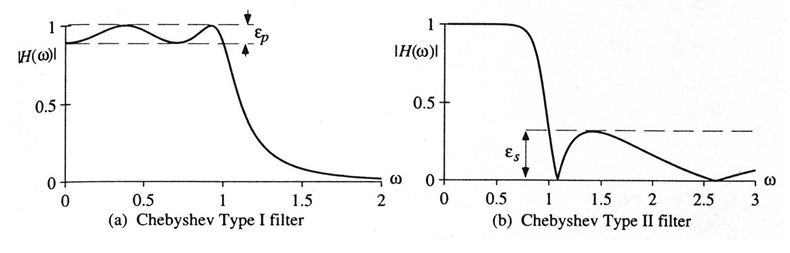
\includegraphics[scale = 1]{Filtri di Chebyshev di ordine 1 e 2.PNG}
\end{figure}  

Un'altra famiglia di filtri sono quelli di Bessel, il cui modulo è costante per tutte le frequenze, ma è molto utile per migliorare la fase. \newline 

\newpage 

\subsection{Esempi di filtri digitali} 

Se il segnale è digitale, quindi non è più analogico, avremo bisogno di filtri digitali, 
quindi non ci saranno più resistori, induttori e condensatori bensì effcienti programmi di calcolo 
chiamati software packages. \newline 

I filtri digitali prendono il nome anche di filtri numerici (in inglese digital filter). \newline 

Un filtro digitale è costituito da: 

\begin{itemize}
    \item x[n], il segnale di ingresso, è costituito da una serie di campioni discreti, estratti da una forma continua alla frequenza di campionamento $f_s$ in cui ogni $x[n_i]$ è contenuto in un regostro
    \item Blocchi $z^{-1}$ che rappresentano un ritardo di simbolo, o periodo di campionamento $T_s = \frac{1}{f_s}$ 
    \item tap, che sono gli elementi di ritardo 
    \item weight, o pesi in italiano, sono i coefficienti che moltiplicano le uscite dei tap 
    \item sommatori (in inglese summing function) che sommano le uscite dei tap pesate dai wieght
\end{itemize} 

Un esempio di filtro digitale: 

\begin{figure}[h]
    \centering
    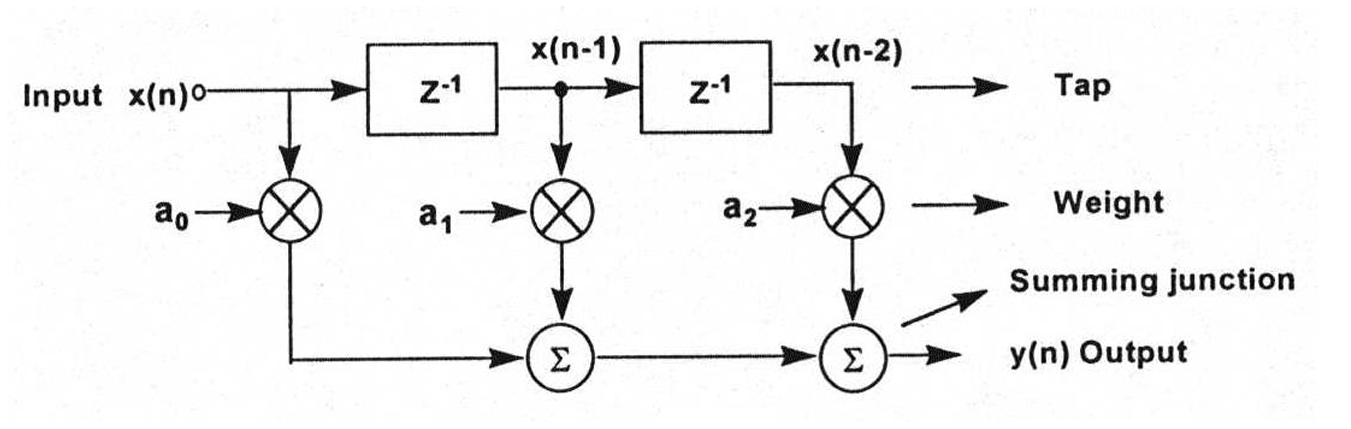
\includegraphics[scale = 0.55]{Esempio di filtro digitale.PNG}
\end{figure}  

La funzione di uscita del filtro di esempio è: 

{
    \Large 
    \begin{equation}
        y[n] = a_0 x[n] + a_1 x[n -1] + a_2 x[n-2]
    \end{equation}
}

Come nel caso analogico, se il filtro è lineare, possiamo esprimere l'uscita di un filtro con la sua risposta impulsiva: 

{
    \Large 
    \begin{equation}
        y[n] = \sum_{\kappa = -\infty}^{\infty} x[n] h[n-k]
    \end{equation}
}

Questa equazione è la convoluzione in digitale, in cui x[n] è la seguenza di ingresso e h[n] è la risposta impulsiva. \newline  

In base alla risposta impulsiva del filtro, possiamo distinguere due categorie di filtri: 

\begin{itemize}
    \item i FIR, Finite Impulse Response 
    \item gli IIR, Infinite Impulse Response 
\end{itemize}

I FIR hanno questo nome perchè la loro risposta impulsiva è finita, quindi la loro uscita è del tipo: 

{
    \Large 
    \begin{equation}
        y[n] = \sum_{\kappa = 0}^{M} b_\kappa x[n - \kappa]
    \end{equation}
}


La loro risposta impulsiva è del tipo: 

{
    \Large 
    \begin{equation}
        h[n] = \sum_{\kappa = 0}^{M} b_\kappa \delta[n - \kappa] = 
        \begin{cases}
            b_n \text{ se } 0 \leq n \leq M \\ 
            0 \text{ altrimenti }
        \end{cases}
    \end{equation}
}

Un filtro in cui la risposta dipende dall'uscita negli istanti precedenti è un filtro ricorsivo, o anche detto IIR. \newline 


I filtri IIR sono, in linea di principio, più efficienti rispetto ai filtri FIR perchè hanno bisogno di meno tap per
avere lo stesso roll-off rate. \newline 

In certi casi, si preferiscono i filtri FIR grazie alla loro caratteristica di essere, per definizione, sempre stabili. \newline 

In generale, maggiori sono i registri, maggiore sarà il tempo di elaborazione. \newline 

\newpage 
. 
\newpage
. 
\newpage